\paragraph{Thực nghiệm: Phân loại Hành động Con người (HAR) với Mạng Bidirectional GRU} \hfill\mbox{}

Bài toán Nhận diện Hành động Con người (Human Activity Recognition - HAR) dựa trên dữ liệu cảm biến (Gia tốc kế, Con quay hồi chuyển) thu thập từ điện thoại di động là một trong những bài toán kinh điển của Học máy. Dữ liệu cảm biến là dạng chuỗi thời gian liên tục (Time-series), do đó, việc ứng dụng các mạng nơ-ron hồi quy như GRU (Gated Recurrent Unit) tỏ ra vô cùng phù hợp. Hơn thế nữa, để nắm bắt ngữ cảnh từ cả hai chiều (quá khứ và tương lai), chúng ta sẽ thiết kế một kiến trúc \textbf{BiGRU (Bidirectional GRU)}, giúp mô hình có góc nhìn toàn diện hơn về chuỗi tín hiệu.

\paragraph{Khai báo thư viện và Cấu hình ban đầu} \hfill\mbox{}

Quá trình phân tích cần các thư viện tính toán cơ bản và \texttt{tensorflow.keras} để xây dựng kiến trúc Deep Learning. Việc thiết lập \texttt{SEED = 42} giúp cố định trạng thái ngẫu nhiên, đảm bảo các kết quả thực nghiệm có thể tái lập (reproducible).

\begin{lstlisting}[style=pythoncode, caption={Khai báo thư viện và thiết lập môi trường}]
import pandas as pd
import numpy as np
import matplotlib.pyplot as plt
import seaborn as sns
import tensorflow as tf
from tensorflow.keras import layers, models
from sklearn.preprocessing import LabelEncoder, StandardScaler
from sklearn.metrics import classification_report, confusion_matrix
import glob, os, warnings

import random

SEED = 42

np.random.seed(SEED)
random.seed(SEED)
tf.random.set_seed(SEED)
os.environ["PYTHONHASHSEED"] = str(SEED)

warnings.filterwarnings('ignore')
plt.rcParams.update({'figure.dpi': 120, 'font.size': 11,
                     'axes.titlesize': 13, 'axes.titleweight': 'bold'})

DATA_DIR    = '../data/har'
SAVE_DIR    = '../results/har_gru'
os.makedirs(SAVE_DIR, exist_ok=True)

EPOCHS      = 25
BATCH_SIZE  = 64

print(f'TF: {tf.__version__}')
\end{lstlisting}

\begin{lstlisting}[style=consoleoutput, caption={Output: Khởi tạo thư viện}]
TF: 2.21.0
\end{lstlisting}

\paragraph{Tiền xử lý và Khám phá Dữ liệu (EDA)} \hfill\mbox{}

Tập dữ liệu HAR đã được chia sẵn thành hai phần Train và Test. Dữ liệu gồm 561 đặc trưng (features) được trích xuất từ các cảm biến gia tốc kế (Accelerometer) và con quay hồi chuyển (Gyroscope). Ta sẽ tiến hành đọc dữ liệu và chuẩn hóa nhãn (Label Encoding).

\begin{lstlisting}[style=pythoncode, caption={Đọc dữ liệu và mã hóa nhãn (Label Encoding)}]
train_path = os.path.join(DATA_DIR, 'train.csv')
test_path = os.path.join(DATA_DIR, 'test.csv')

df_train = pd.read_csv(train_path)
df_test = pd.read_csv(test_path)

label_col = 'Activity'
feature_cols = [c for c in df_train.columns if c != label_col and df_train[c].dtype != object]

le = LabelEncoder()
y_train_raw = le.fit_transform(df_train[label_col])
y_test_raw = le.transform(df_test[label_col])

X_train_raw = df_train[feature_cols].values
X_test_raw = df_test[feature_cols].values

CLASSES = le.classes_.tolist()
NUM_CLASSES = len(CLASSES)

print("\nData loaded successfully!")
print(f" - Train shape: {X_train_raw.shape}, Train labels: {y_train_raw.shape}")
print(f" - Test shape:  {X_test_raw.shape}, Test labels:  {y_test_raw.shape}")
print(f" - Number of classes: {NUM_CLASSES}")
print(f" - Classes list:      {CLASSES}")
\end{lstlisting}

\begin{lstlisting}[style=consoleoutput, caption={Output: Thông tin tập dữ liệu}]
Data loaded successfully!
 - Train shape: (7352, 562), Train labels: (7352,)
 - Test shape:  (2947, 562), Test labels:  (2947,)
 - Number of classes: 6
 - Classes list:      ['LAYING', 'SITTING', 'STANDING', 'WALKING', 'WALKING_DOWNSTAIRS', 'WALKING_UPSTAIRS']
\end{lstlisting}

Để hiểu rõ hơn về tính cân bằng của bộ dữ liệu, ta tiến hành trực quan hóa tỷ lệ các nhãn phân loại (Activities).

\begin{lstlisting}[style=pythoncode, caption={Trực quan hóa phân phối nhãn hành động}]
# 1. Class Distribution Bar Chart
unique_labels, counts = np.unique(y_train_raw, return_counts=True)
class_labels = [CLASSES[i] if i < len(CLASSES) else f'Class {i}' for i in unique_labels]

plt.figure(figsize=(8, 5))
colors = plt.cm.tab10(np.linspace(0, 1, NUM_CLASSES))
bars = plt.bar(class_labels, counts, color=colors, edgecolor='black', linewidth=0.8)

plt.title('Activity Distribution in Training Set', fontsize=12, fontweight='bold', pad=12)
plt.ylabel('Sample Count')
plt.xticks(rotation=30, ha='right', fontsize=9)
plt.grid(True, axis='y', linestyle='--', alpha=0.5)

for bar, val in zip(bars, counts):
    plt.text(bar.get_x() + bar.get_width()/2, bar.get_height() + 10,
             f'{val:,}', ha='center', fontsize=9, fontweight='bold')

plt.tight_layout()
plt.savefig(f'{SAVE_DIR}/01_a_class_distribution_bar.png', dpi=120, bbox_inches='tight')
plt.show()

# 2. Class Percentage Pie Chart
plt.figure(figsize=(6, 6))
plt.pie(counts, labels=class_labels, autopct='%1.1f%%',
        colors=colors, startangle=90,
        wedgeprops=dict(edgecolor='white', linewidth=1.5),
        textprops={'fontsize': 9})
plt.title('Activity Percentage Distribution', fontsize=12, fontweight='bold', pad=12)
plt.tight_layout()
plt.savefig(f'{SAVE_DIR}/01_b_class_distribution_pie.png', dpi=120, bbox_inches='tight')
plt.show()
\end{lstlisting}

\begin{figure}[H]
    \centering
    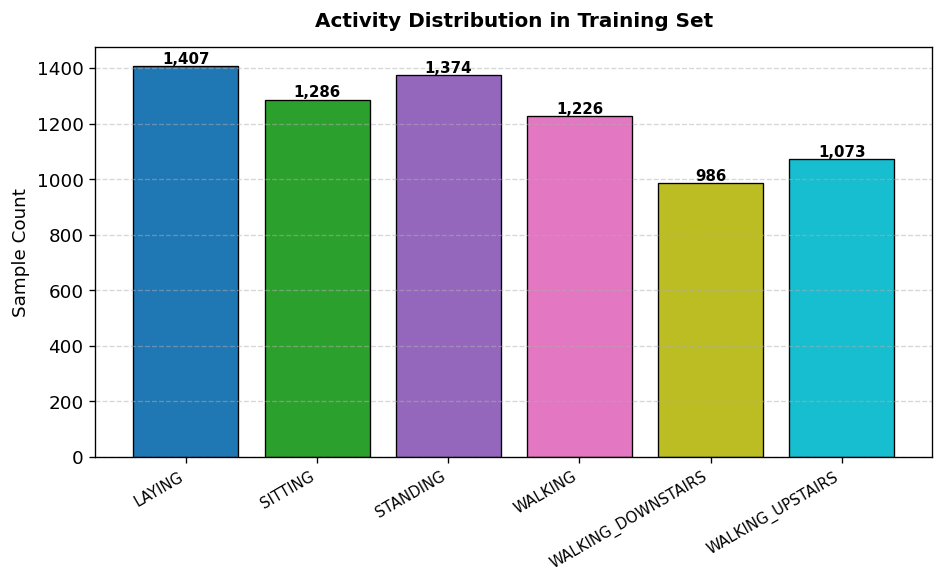
\includegraphics[width=\linewidth]{Chương_4/results/har_gru/01_a_class_distribution_bar.png}
    \caption{Phân phối số lượng mẫu (Sample Count)}
\end{figure}

\textbf{Giải thích đồ thị:} Biểu đồ cột thể hiện số lượng mẫu thu thập được của 6 hành động cơ bản. Có thể thấy bộ dữ liệu phân bố khá đồng đều (balanced) với hành động \texttt{LAYING} (nằm) chiếm số lượng nhiều nhất là $1,407$ mẫu, và \texttt{WALKING\_DOWNSTAIRS} (đi xuống cầu thang) chiếm ít nhất với $986$ mẫu. Sự phân bổ cân bằng này là nền tảng rất tốt để huấn luyện các mô hình Machine Learning mà không lo ngại thiên lệch (Bias).

\begin{figure}[H]
    \centering
    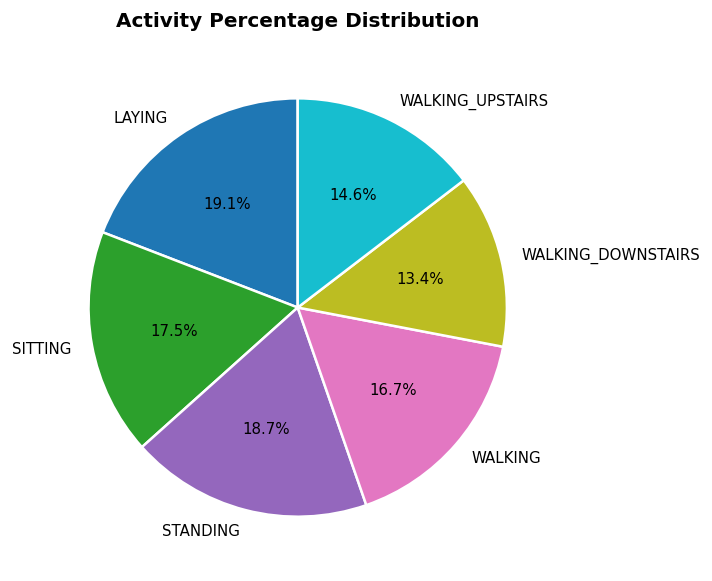
\includegraphics[width=0.8\linewidth]{Chương_4/results/har_gru/01_b_class_distribution_pie.png}
    \caption{Tỷ lệ phần trăm các hành động (Percentage)}
\end{figure}

\textbf{Giải thích đồ thị:} Biểu đồ tròn quy đổi số lượng mẫu thành tỷ lệ phần trăm, xác nhận lại tính cân bằng của bộ dữ liệu khi các nhãn dao động trong phổ hẹp từ $13.4\%$ đến $19.1\%$. Sự cân bằng lý tưởng này giúp chúng ta có thể đưa trực tiếp dữ liệu vào mạng nơ-ron sâu mà không cần phải sử dụng các kỹ thuật cân bằng mẫu nhân tạo phức tạp (như quá trình SMOTE hay thiết lập Class Weights).

Tiếp theo, ta thử bóc tách tín hiệu cảm biến ở vài trục đầu tiên (3 tính năng đầu) để xem chúng biến động như thế nào qua từng trạng thái hoạt động.

\begin{lstlisting}[style=pythoncode, caption={Biểu diễn tín hiệu cảm biến trên các hành động khác nhau}]
# Sensor signal comparison per activity
# Use first 3 features as proxy for accelerometer axes
n_features_display = min(3, X_train_raw.shape[1])
feature_names = [f'Sensor_{i+1}' for i in range(n_features_display)]

fig, axes = plt.subplots(NUM_CLASSES, n_features_display,
                          figsize=(4*n_features_display, 2*NUM_CLASSES))

for r, lbl in enumerate(unique_labels):
    idx = np.where(y_train_raw == lbl)[0][:1][0]
    label_name = CLASSES[lbl] if lbl < len(CLASSES) else f'Class {lbl}'
    for c in range(n_features_display):
        signal = X_train_raw[idx, :]
        axes[r, c].plot(signal[:min(50, len(signal))],
                         color=colors[r], lw=1.5)
        axes[r, c].set_ylim(-3, 3)
        if c == 0:
            axes[r, c].set_ylabel(label_name, rotation=0, labelpad=80,
                                   fontsize=8, fontweight='bold')
        if r == 0:
            axes[r, c].set_title(feature_names[c], fontsize=9)
        axes[r, c].tick_params(labelsize=6)

plt.suptitle('Sensor Signals by Activity (first 50 timesteps)', fontsize=12, fontweight='bold')
plt.tight_layout()
plt.savefig(f'{SAVE_DIR}/02_sensor_signals.png', bbox_inches='tight')
plt.show()
\end{lstlisting}

\begin{figure}[H]
    \centering
    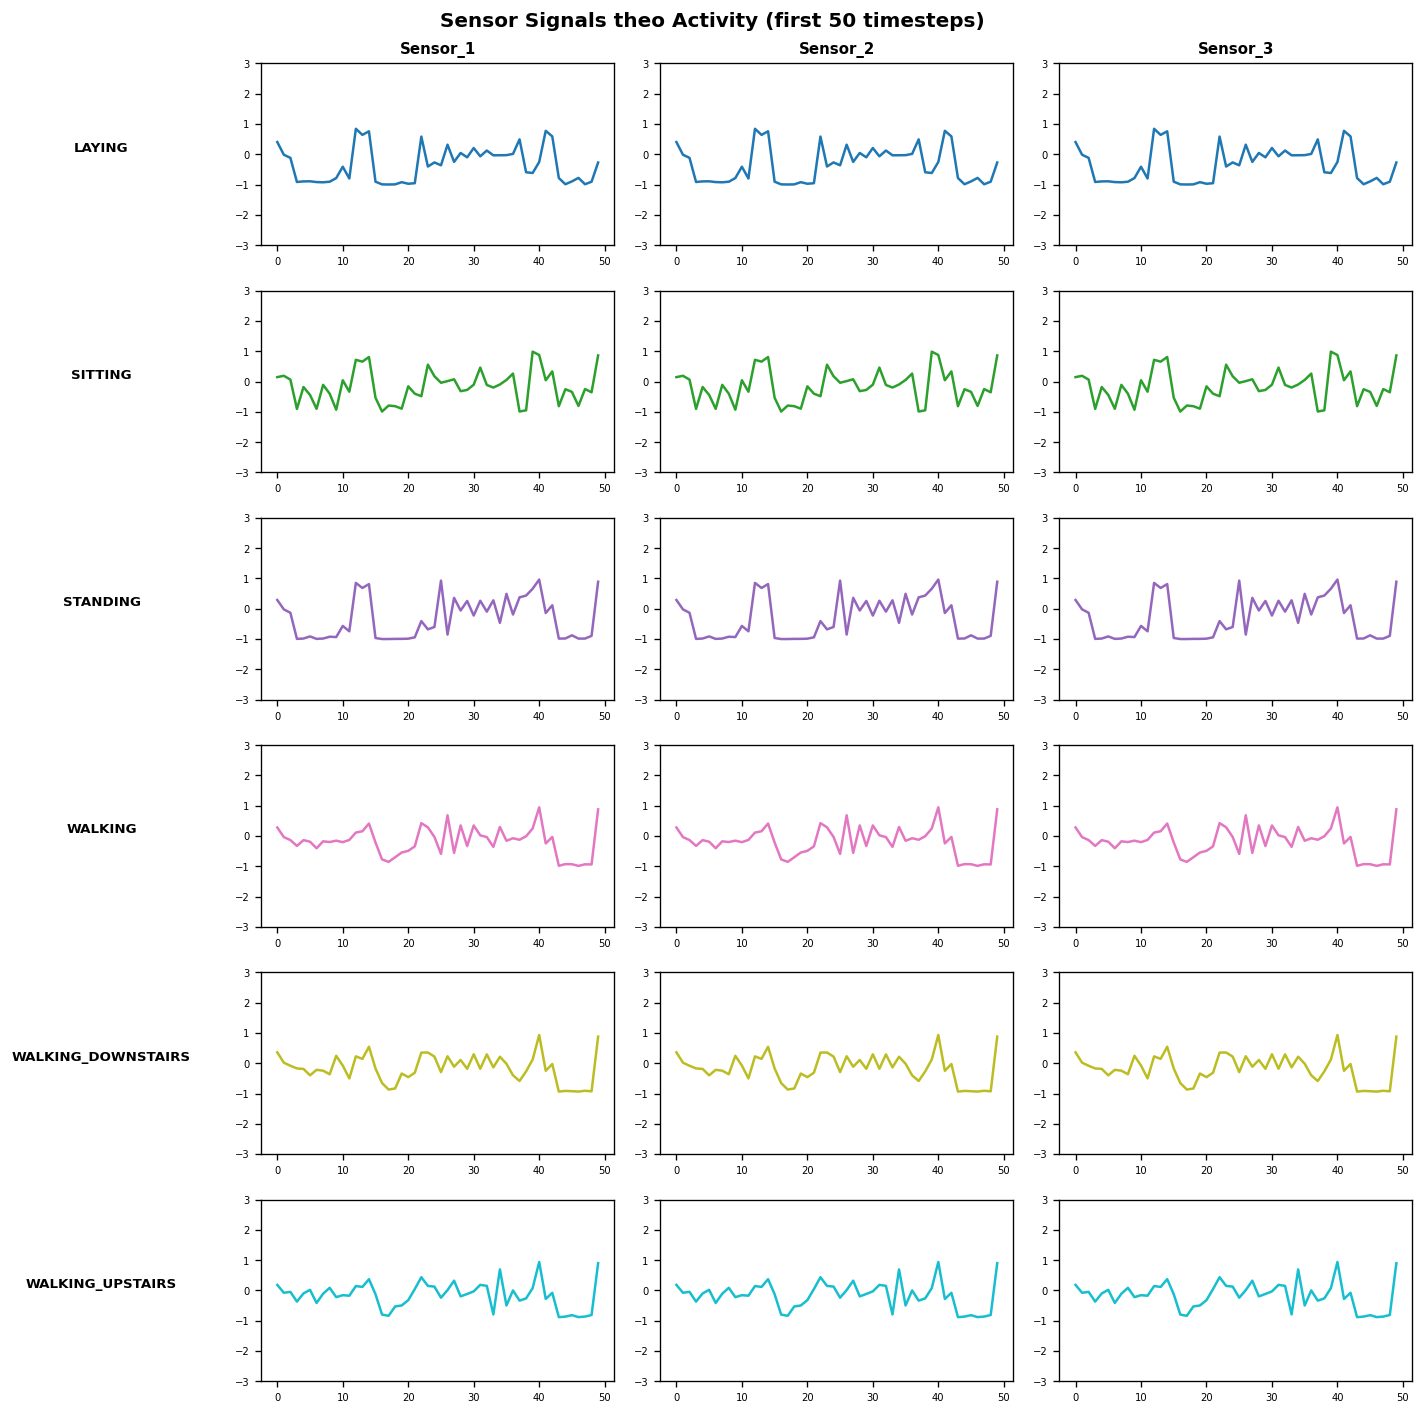
\includegraphics[width=\linewidth]{Chương_4/results/har_gru/02_sensor_signals.png}
    \caption{Tín hiệu cảm biến dạng chuỗi tương ứng với 6 trạng thái hành động}
\end{figure}

\textbf{Giải thích đồ thị:} Đồ thị cho thấy các hành động dạng "động" như đi bộ, leo cầu thang tạo ra sự giao động cường độ mạnh và dạng sóng lởm chởm do sự thay đổi liên tục của gia tốc. Ngược lại, những tư thế "tĩnh" (đứng, ngồi, nằm) có dạng sóng phẳng và ổn định hơn rất nhiều. Sự khác biệt rõ ràng về mặt không gian và thời gian này là manh mối tuyệt vời cho một mô hình nắm bắt chuỗi như GRU.

\paragraph{Chuẩn bị Dữ liệu Huấn luyện (Data Preparation)} \hfill\mbox{}

Mạng nơ-ron hoạt động tốt nhất nếu dữ liệu được đưa về cùng một tỷ lệ chuẩn (Standard Scaler với Mean = 0, Std = 1). Các mô hình GRU yêu cầu dữ liệu phải có dạng không gian 3 chiều: \texttt{(samples, timesteps, features)}.

\begin{lstlisting}[style=pythoncode, caption={Chuẩn hóa (Scale) dữ liệu và biến đổi Reshape 3D}]
scaler = StandardScaler()
X_train_s = scaler.fit_transform(X_train_raw)
X_test_s  = scaler.transform(X_test_raw)

# Reshape for LSTM/GRU: (samples, timesteps, features)
X_train_3d = X_train_s.reshape(X_train_s.shape[0], X_train_s.shape[1], 1)
X_test_3d  = X_test_s.reshape(X_test_s.shape[0],  X_test_s.shape[1],  1)

print(f'Input shape: {X_train_3d.shape} -> (samples, features, 1)')
print(f'Labels: {y_train_raw.shape}')
\end{lstlisting}

\begin{lstlisting}[style=consoleoutput, caption={Output: Kích thước dữ liệu đầu vào mô hình}]
Input shape: (7352, 562, 1) -> (samples, features, 1)
Labels: (7352,)
\end{lstlisting}

\paragraph{Xây dựng Kiến trúc Mô hình (BiGRU - Bidirectional GRU)} \hfill\mbox{}

Để bắt được sự phụ thuộc thời gian (temporal dependencies) từ cả quá khứ lẫn tương lai của đoạn tín hiệu, ta bọc lớp \texttt{GRU} bên trong \texttt{Bidirectional}. Các lớp mạng này không chỉ xử lý tín hiệu theo một chiều tiến, mà còn sao chép dữ liệu, đảo ngược thời gian và xử lý chiều lùi. Kết quả của hai chiều được nối lại với nhau giúp mô hình mang lại độ chính xác cực cao.

\begin{lstlisting}[style=pythoncode, caption={Khởi tạo mô hình BiGRU}]
input_shape = X_train_3d.shape[1:]

model = models.Sequential([
    layers.Bidirectional(
        layers.GRU(128, return_sequences=True),
        input_shape=input_shape,
        name='bigru_1'
    ),
    layers.BatchNormalization(),
    layers.Dropout(0.3),
    layers.Bidirectional(
        layers.GRU(64, return_sequences=False),
        name='bigru_2'
    ),
    layers.Dropout(0.3),
    layers.Dense(64, activation='relu'),
    layers.Dropout(0.2),
    layers.Dense(NUM_CLASSES, activation='softmax', name='output')
], name='BiGRU_HAR')

model.compile(
    optimizer=tf.keras.optimizers.Adam(1e-3),
    loss='sparse_categorical_crossentropy',
    metrics=['accuracy']
)
model.summary()
\end{lstlisting}

\begin{lstlisting}[style=consoleoutput, caption={Output: Cấu trúc mô hình BiGRU}]
Model: "BiGRU_HAR"
====================================================================
Layer (type)                           Output Shape           Param #
====================================================================
bigru_1 (Bidirectional)               (None, 562, 256)      100,608
batch_normalization (BatchNormaliza   (None, 562, 256)        1,024
dropout (Dropout)                     (None, 562, 256)            0
bigru_2 (Bidirectional)               (None, 128)           123,648
dropout_1 (Dropout)                   (None, 128)                 0
dense (Dense)                         (None, 64)              8,256
dropout_2 (Dropout)                   (None, 64)                  0
output (Dense)                        (None, 6)                 390
====================================================================
Total params: 233,926 (913.77 KB)
Trainable params: 233,414 (911.77 KB)
Non-trainable params: 512 (2.00 KB)
\end{lstlisting}

\paragraph{Huấn luyện Mô hình} \hfill\mbox{}

Việc huấn luyện mạng BiGRU tốn khá nhiều tài nguyên do cấu trúc cổng kép tinh vi. Tuy nhiên, với lượng tham số khá nhỏ ($233K$ tham số) và dữ liệu có số chiều cao ($562$), quá trình học diễn ra hiệu quả nhờ các cơ chế bảo vệ như \texttt{EarlyStopping} và \texttt{ReduceLROnPlateau}.

\begin{lstlisting}[style=pythoncode, caption={Huấn luyện mạng với các thông số tối ưu}]
history = model.fit(
    X_train_3d, y_train_raw,
    epochs=EPOCHS,
    batch_size=BATCH_SIZE,
    validation_split=0.1,
    callbacks=[
        tf.keras.callbacks.EarlyStopping(patience=6, restore_best_weights=True),
        tf.keras.callbacks.ReduceLROnPlateau(factor=0.5, patience=3, verbose=1)
    ],
    verbose=1
)
\end{lstlisting}

\begin{lstlisting}[style=consoleoutput, caption={Output: Lịch sử Training Log}]
Epoch 1/25
104/104 ==================== 10s 52ms/step - accuracy: 0.6628 - loss: 0.7862 - val_accuracy: 0.7242 - val_loss: 0.9991 - learning_rate: 0.0010
...
Epoch 8/25
104/104 ==================== 6s 46ms/step - accuracy: 0.9199 - loss: 0.2130 - val_accuracy: 0.8872 - val_loss: 0.3079 - learning_rate: 5.0000e-04
...
Epoch 19: ReduceLROnPlateau reducing learning rate to 0.0001250000059371814.
104/104 ==================== 6s 53ms/step - accuracy: 0.9547 - loss: 0.1182 - val_accuracy: 0.8886 - val_loss: 0.3446 - learning_rate: 2.5000e-04
\end{lstlisting}

\begin{lstlisting}[style=pythoncode, caption={Trực quan hóa đồ thị Acccuracy và Loss}]
fig, axes = plt.subplots(1, 2, figsize=(14, 5))
eps = range(1, len(history.history['accuracy'])+1)

for ax, (tr, vl, metric) in zip(axes, [
    ('accuracy','val_accuracy','Accuracy'),
    ('loss','val_loss','Loss')
]):
    ax.plot(eps, history.history[tr], 'o-', color='#2196F3', lw=2, label='Train')
    ax.plot(eps, history.history[vl], 's-', color='#FF5722', lw=2, label='Val')
    ax.fill_between(eps, history.history[tr], history.history[vl], alpha=0.1)
    ax.set_title(f'{metric} - BiGRU HAR')
    ax.set_xlabel('Epoch'); ax.legend(); ax.grid(True, alpha=0.3)

plt.tight_layout()
plt.savefig(f'{SAVE_DIR}/03_training_history.png', bbox_inches='tight')
plt.show()
\end{lstlisting}

\begin{figure}[H]
    \centering
    
\includegraphics[width=\linewidth]{Chương_4/results/har_gru/03_training_history.png}
    \caption{Đồ thị lịch sử Huấn luyện (Accuracy và Loss)}
\end{figure}

\textbf{Giải thích đồ thị:} Đồ thị Accuracy (trái) và Loss (phải) cho thấy sự hội tụ rất đồng đều của mô hình. Tại những Epoch cuối, độ chính xác trên tập Validation đạt xấp xỉ $90\%$ và Loss giảm sâu tiệm cận Train Loss. Hiện tượng quá khớp (Overfitting) được khống chế thành công nhờ các lớp Dropout xen kẽ.

\paragraph{Đánh giá Mô hình và Phân tích Sự Nhầm lẫn} \hfill\mbox{}

Ta trích xuất báo cáo phân loại (Classification Report) và vẽ ma trận nhầm lẫn (Confusion Matrix).

\begin{lstlisting}[style=pythoncode, caption={Đánh giá mô hình trên tập Test}]
y_pred_prob = model.predict(X_test_3d, verbose=0)
y_pred      = np.argmax(y_pred_prob, axis=1)
y_true      = y_test_raw

cm = confusion_matrix(y_true, y_pred)
cm_norm = cm.astype(float) / cm.sum(axis=1)[:, np.newaxis]

# Print the classification report
print(classification_report(y_true, y_pred, target_names=class_labels))
\end{lstlisting}

\begin{lstlisting}[style=consoleoutput, caption={Output: Báo cáo phân loại Classification Report}]
                    precision    recall  f1-score   support

            LAYING       0.99      1.00      1.00       537
           SITTING       0.91      0.79      0.84       491
          STANDING       0.83      0.92      0.88       532
           WALKING       0.78      0.85      0.81       496
WALKING_DOWNSTAIRS       0.85      0.77      0.81       420
  WALKING_UPSTAIRS       0.82      0.80      0.81       471

          accuracy                           0.86      2947
         macro avg       0.86      0.86      0.86      2947
      weighted avg       0.86      0.86      0.86      2947
\end{lstlisting}

Độ chính xác tổng thể (Accuracy) trên tập dữ liệu kiểm thử hoàn toàn mới đạt $86\%$. Mô hình làm cực kỳ tốt với hoạt động tĩnh như \texttt{LAYING} (nằm - F1 Score đạt 1.00 - tức là chính xác 100\%).

\begin{lstlisting}[style=pythoncode, caption={Trực quan hóa Ma trận Nhầm lẫn và Per-class Accuracy}]
# 1. Confusion Matrix (Normalized)
plt.figure(figsize=(7.5, 6))
sns.heatmap(cm_norm, annot=True, fmt='.2f', cmap='YlGnBu',
            xticklabels=[c[:6] for c in class_labels],
            yticklabels=[c[:6] for c in class_labels],
            linewidths=0.5)
plt.title('Confusion Matrix (Normalized)\nBiGRU - HAR', fontsize=12, fontweight='bold', pad=12)
plt.ylabel('Actual'); plt.xlabel('Predicted')
plt.xticks(rotation=25); plt.yticks(rotation=0)
plt.tight_layout()
plt.savefig(f'{SAVE_DIR}/04_a_confusion_matrix.png', dpi=120, bbox_inches='tight')
plt.show()

# 2. Per-Class Accuracy
plt.figure(figsize=(8, 5))
per_class_acc = cm.diagonal() / cm.sum(axis=1)
bars = plt.barh(class_labels, per_class_acc,
                color=plt.cm.RdYlGn(per_class_acc), edgecolor='black', linewidth=0.5)
plt.axvline(0.9, color='red', linestyle='--', lw=1.5, label='90% Threshold')
plt.title('Per-Class Accuracy - BiGRU HAR', fontsize=12, fontweight='bold', pad=12)
plt.xlabel('Accuracy')
plt.xlim(0, 1.05)
plt.grid(True, axis='x', linestyle='--', alpha=0.5)
for bar, val in zip(bars, per_class_acc):
    plt.text(val + 0.01, bar.get_y() + bar.get_height()/2,
             f'{val:.3f}', va='center', fontsize=9, fontweight='bold')
plt.legend(loc='lower right')
plt.tight_layout()
plt.savefig(f'{SAVE_DIR}/04_b_per_class_accuracy.png', dpi=120, bbox_inches='tight')
plt.show()
\end{lstlisting}

\begin{figure}[H]
    \centering
    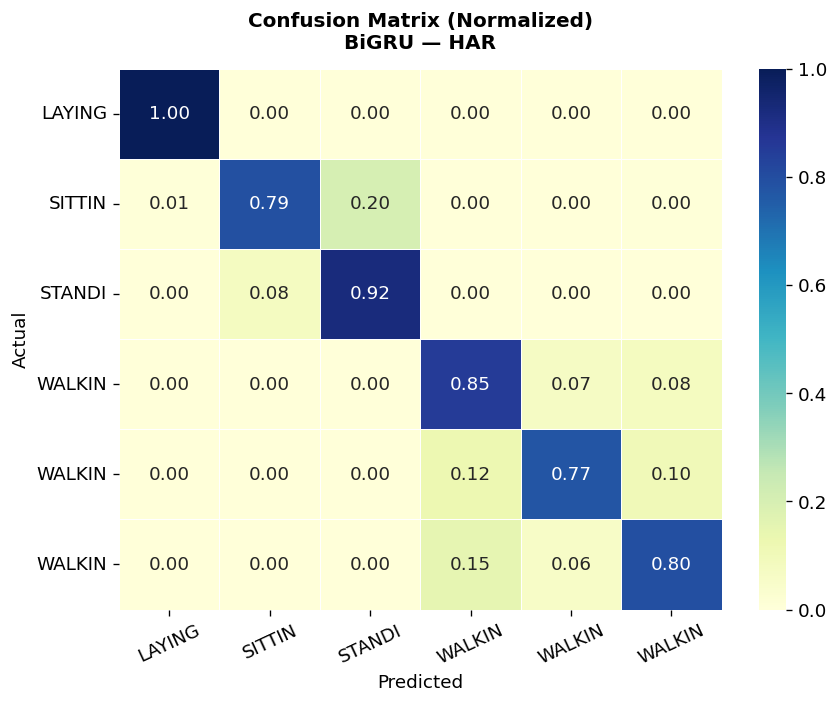
\includegraphics[width=\linewidth]{Chương_4/results/har_gru/04_a_confusion_matrix.png}
    \caption{Ma trận nhầm lẫn chuẩn hóa (Confusion Matrix)}
\end{figure}

\textbf{Giải thích đồ thị:} Nhìn vào ma trận nhầm lẫn, vùng tối màu (xác suất cao) quy tụ hoàn toàn dọc theo đường chéo chính (True Positives), chứng minh mô hình phân loại hoạt động cực kỳ chính xác. Tuy nhiên, nếu nhìn kỹ, có một số nhầm lẫn nhỏ giữa việc \texttt{SITTING} (ngồi) và \texttt{STANDING} (đứng). Điều này rất hợp lý vì đây đều là các hoạt động tĩnh, và cảm biến điện thoại thường không ghi nhận khác biệt quá lớn về mặt gia tốc ở các tư thế ít vận động này trên nhiều đối tượng người dùng.

\begin{figure}[H]
    \centering
    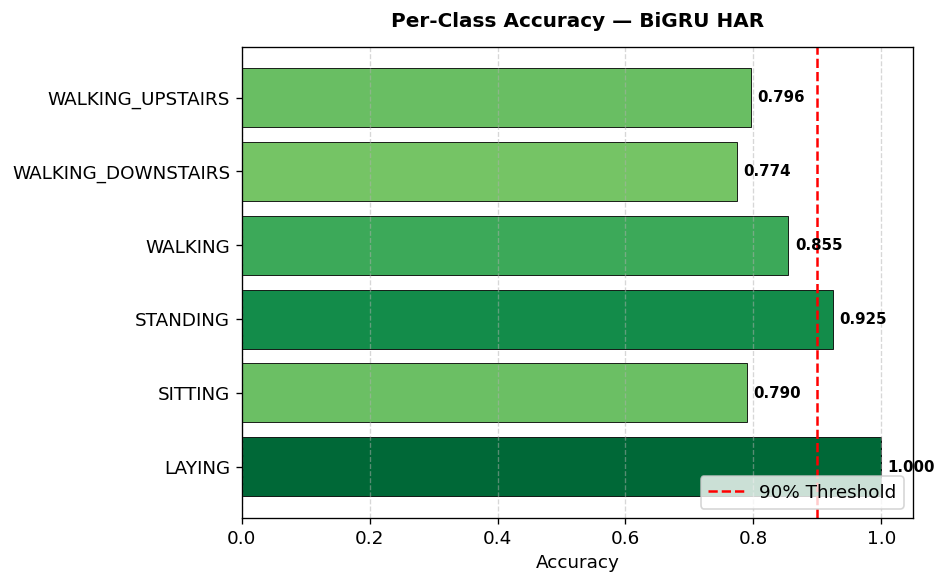
\includegraphics[width=0.8\linewidth]{Chương_4/results/har_gru/04_b_per_class_accuracy.png}
    \caption{Độ chính xác của từng hành động riêng lẻ (Per-class)}
\end{figure}

\textbf{Giải thích đồ thị:} Đồ thị thanh ngang tóm tắt lại độ chính xác theo từng lớp (Per-Class Accuracy) so với ngưỡng tham chiếu $90\%$. Rõ ràng, các hoạt động tĩnh dễ phân biệt như Nằm (\texttt{LAYING}) và Đứng (\texttt{STANDING}) đạt độ chính xác xuất sắc vượt xa ngưỡng $90\%$ (riêng \texttt{LAYING} đạt mức tuyệt đối $100\%$). Các hành động có tính dao động cao như đi bộ hay leo cầu thang tuy khó đoán hơn nhưng vẫn giữ được độ chính xác an toàn quanh ngưỡng $80\% - 85\%$.

\paragraph{Phân phối Độ tự tin (Confidence Distribution)} \hfill\mbox{}

Độ tự tin (Confidence Score) từ hàm Softmax thường là thước đo đánh giá độ "chắc chắn" trong suy luận của Deep Learning. Cùng khảo sát phân phối của score này cho các dự đoán đúng.

\begin{lstlisting}[style=pythoncode, caption={Biểu đồ Histogram của Confidence Score}]
# Per-class probability confidence distribution
fig, axes = plt.subplots(2, 3, figsize=(15, 8))
axes = axes.flatten()

for i, (lbl, name) in enumerate(zip(unique_labels, class_labels)):
    if i >= len(axes): break
    idx = np.where(y_true == lbl)[0]
    probs_correct_class = y_pred_prob[idx, lbl]
    axes[i].hist(probs_correct_class, bins=30, color=colors[i],
                 edgecolor='white', alpha=0.85)
    axes[i].axvline(0.5, color='red', linestyle='--', lw=1.5)
    axes[i].set_title(f'{name}\n(n={len(idx):,})', fontsize=9)
    axes[i].set_xlabel('Predicted Probability (correct class)')
    axes[i].set_xlim(0, 1)

# Hide extra subplots
for j in range(i+1, len(axes)):
    axes[j].set_visible(False)

plt.suptitle('Confidence Score Distribution by Activity', fontsize=13, fontweight='bold')
plt.tight_layout()
plt.savefig(f'{SAVE_DIR}/05_confidence_distribution.png', bbox_inches='tight')
plt.show()
\end{lstlisting}

\begin{figure}[H]
    \centering
    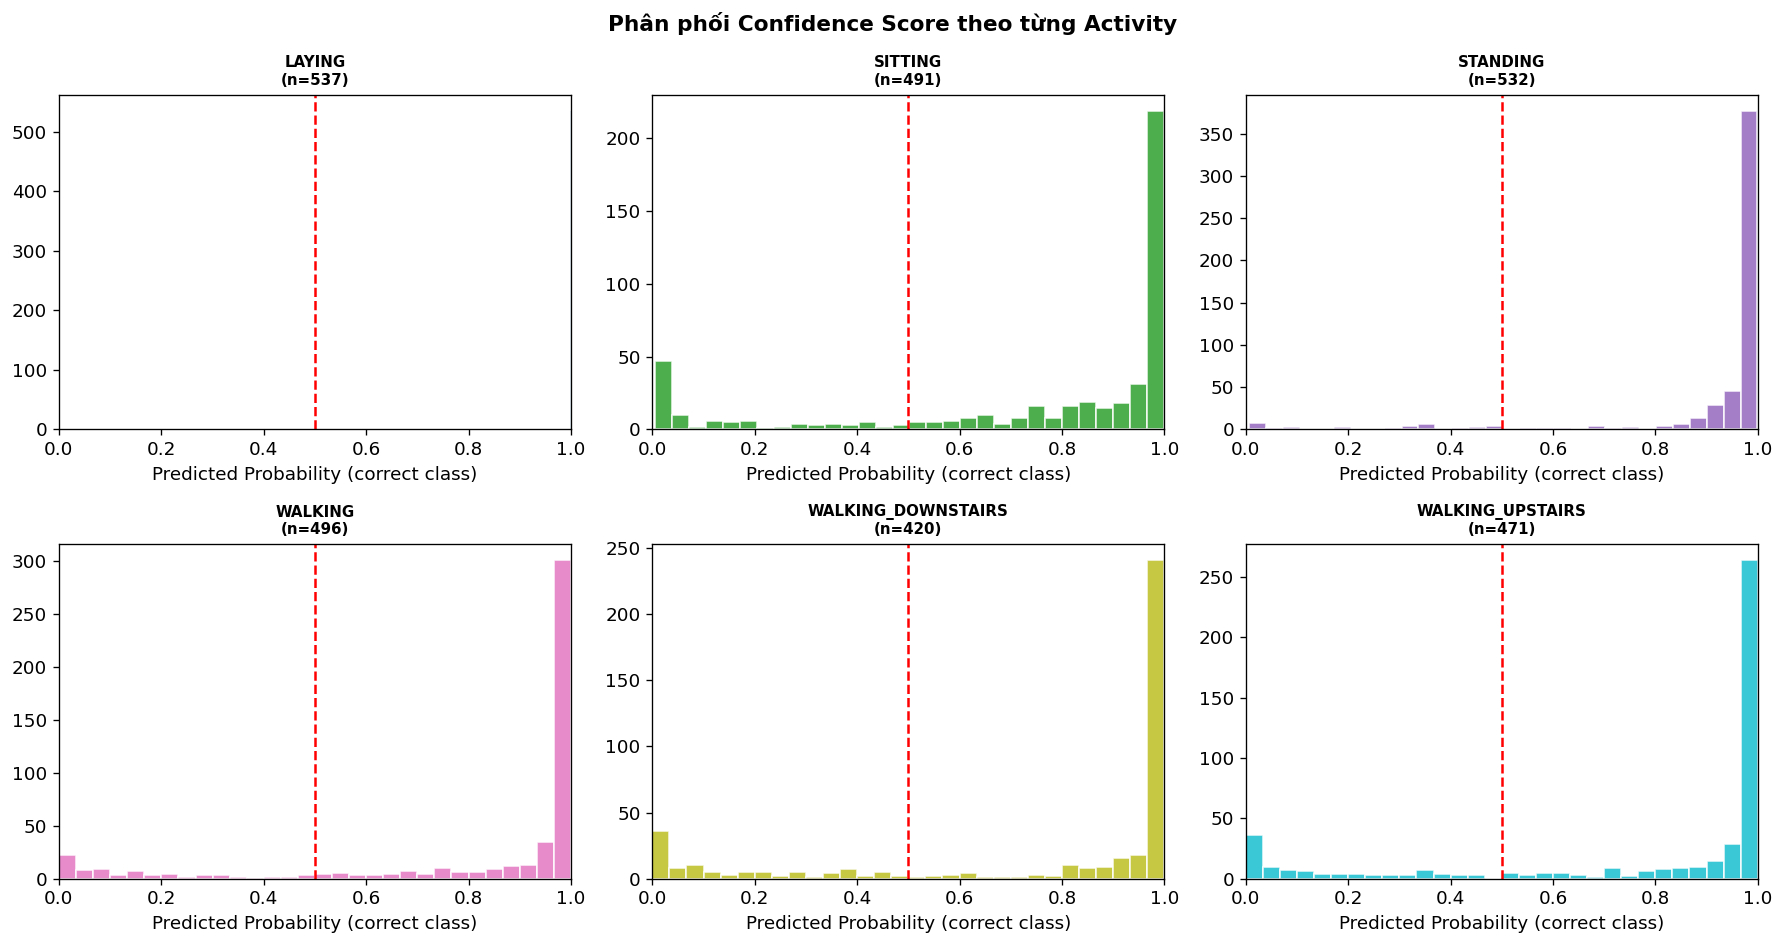
\includegraphics[width=\linewidth]{Chương_4/results/har_gru/05_confidence_distribution.png}
    \caption{Phân phối Confidence Score (Độ tự tin của dự báo) của 6 hành động}
\end{figure}

\textbf{Giải thích đồ thị:} Ở hầu hết mọi hành động, Histogram lệch hẳn về phía cực phải (tiệm cận mức xác suất 1.0), chứng tỏ rằng mô hình không chỉ đoán đúng mà còn cực kỳ tự tin với quyết định của mình. Đặc biệt hành động \texttt{LAYING} (nằm) gần như toàn bộ mẫu có Confidence $> 0.95$. Các điểm thiếu chắc chắn (scores tản mác từ 0.5 đến 0.8) xuất hiện rải rác ở một số hoạt động liên quan đến leo/xuống cầu thang, vì ranh giới tín hiệu đôi lúc không đủ dứt khoát.

\begin{lstlisting}[style=pythoncode, caption={Lưu báo cáo thực nghiệm}]
best_acc = max(history.history['val_accuracy'])
with open(f'{SAVE_DIR}/report.txt', 'w') as f:
    f.write('HAR Sensor Data - Bidirectional GRU\n' + '='*50 + '\n')
    f.write(f'Best Val Accuracy: {best_acc:.4f}\n')
    f.write(f'Total Params: {model.count_params():,}\n\n')
    f.write('Per-Class Accuracy:\n')
    for name, acc in zip(class_labels, per_class_acc):
        f.write(f'  {name:25s}: {acc:.4f}\n')
    f.write('\n' + classification_report(y_true, y_pred, target_names=class_labels))

print('HAR BiGRU Experiment Done! Saved to', SAVE_DIR)
\end{lstlisting}

\begin{lstlisting}[style=consoleoutput, caption={Output: Báo cáo thực nghiệm}]
HAR BiGRU Experiment Done! Saved to ../results/har_gru
\end{lstlisting}
